\documentclass{article}
\textwidth=6in
\hoffset=0in
\voffset=0in

\usepackage{afterpage}
\usepackage{pgf}
\usepackage{tikz}
\usepackage{pdflscape}
\usetikzlibrary{arrows,automata}
\usepackage[latin1]{inputenc}
\usepackage{ngerman}
\usepackage[a4paper, total={6in, 8in}]{geometry}
\usepackage{amsmath}
\usepackage{amssymb}
\usepackage{stmaryrd}
\usepackage{graphicx}
\usepackage{tikz}
\usetikzlibrary{automata, arrows, fit, calc}
\usepackage{pifont}
\usepackage{amssymb}
\usepackage{gensymb}
\usepackage[ampersand]{easylist}


\newcommand{\gap}{\ \\ \\}
\newcommand{\chart}[6]{
    \node[round, 
          minimum width=#5, 
          minimum height=#6] (#1) at (#3,#4) {chart};
    \node[rect] (#2) at (#3,#4) {title};
}
\newcommand{\sepline}[2]{
}

% needs to be updated
\author{Max Springenberg, 177792\\
        Daniel Sonnabend, 190748}
\title{\
    ES "Ubungsblatt 3\\
    Gruppe Fr. 8-10
    }
\setcounter{section}{3}
\date{}

\begin{document}

\maketitle
\newpage

\subsection{Java}

\begin{tabular}{|p{7cm}|p{7cm}|}
	\hline
	
	Vorteile 						        & Nachteile\\
    \hline
    Saubere und sichere Programmiersprache  & Lirbaries sind recht gro"s, 
                                              beannspruchen viel Speicher\\
    \hline
    Unterst"utzung von Multithreading       & Kein direkter Zugang zu 
                                              spezifischen Hardware-Features\\
    \hline
    Platform unabh"angig                    & Garbage-Collector nicht absehbar
                                              , bzw. Unvorhersehbarkeit der Zeit
                                              zu der der Garbage-Collector
                                              eingesetzt wird macht das System
                                              `non-deterministic`.\\
    \hline
                                            & `non-deterministic` dispatcher,
                                               mehrere Methoden mit gleichem
                                               Namen sind zul"assig und Methoden
                                               k"onnen "uberschrieben werden.\\
    \hline
                                            & Daraus resultierende Performanz
                                              Probleme.\\
    \hline
                                            & "Uberpr"ufen von 
                                              Echtzeitanforderungen ist schwer
                                              m"oglich.\\
    \hline
\end{tabular}


\subsection{Aliasing}
Bei Aliasing werden zwei unterschiedliche Signale als gleich interpretiert, 
    weil die Samplingrate nicht frequent/ gro"s genug ist.\\
\\
Es gilt:\\$$
    p_s < 0,5 * p_N,\  
    f_s > 2* f_N$$
, wobei $f_s$ die Samplingrate ist.\\
Daraus folgt f"ur unser Beispiel $2*f_N = 2 * 20Hz = 40Hz$, also m"ussen wir
    eine Samplingrate von gr"o"ser $40Hz$  benuzten.\\

\subsection{SDF vs. Petrinetze}
SDFs modelieren den Data-Flow, also wie Daten durch das System flie"sen sollen
    und Petrinetze modelieren kausale Abh"angigkeiten zwischen Ereignissen,
    also was eingetreten sein muss, bevor ein Ereigniss statt finden kann.\\
\\
In einem Petri-Netz spielt Zeit eine Untergeordnete Rolle, die Ordnung in der
    Transitionen `feuern` ist nicht fix. Das macht Petrinetze 
    nichtdeterministisch.\\
\\
Aus einem SDF kann Code generiert werden, bzw. eine Umwandlung zwischen dem
    Modell in Code ist m"oglich. Dies ist bei Petrinetzen nicht der Fall, weil
    das Modell in sich korrekt sein kann, dies aber nicht zwingend auf das 
    ganze System "ubertragbar sein muss.\\

\subsection{Successive-Approximation-Register}
%wie in 30/31 (3.1), nur mit 8, statt 4 BIt/ Ausg"angen.\\
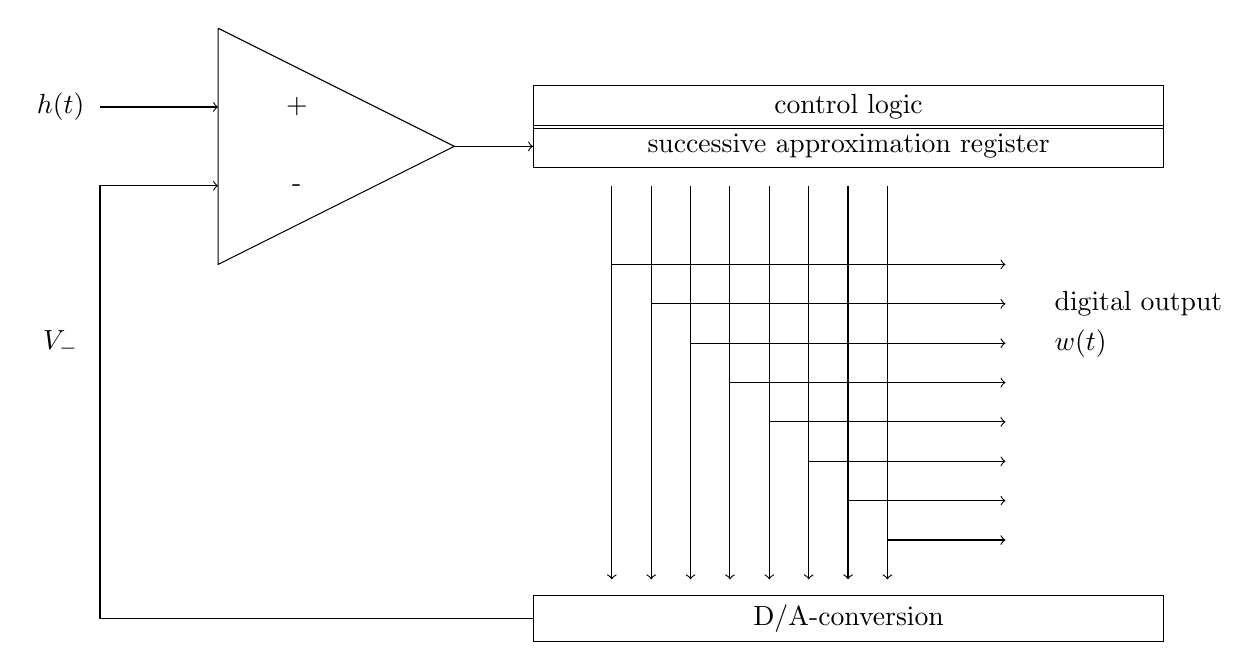
\begin{tikzpicture}
    \node[] (ht) at (0,0) {$h(t)$};
    \node[] (V-) at (0,-3) {$V_-$};
    \node[] (+) at (3,0)  {+};
    \node[] (-) at (3,-1) {-};
    \draw[-] (2,1) coordinate to (5,-0.5) to (2,-2) to (2,1);
    \node[draw, minimum width=8cm,anchor=west] 
         (ctrlgc) at (6,0) {control logic};
    \node[draw, minimum width=8cm,anchor=west] 
         (sar) at (6,-0.5) {successive approximation register};
    \node[draw, minimum width=8cm,anchor=west] 
         (da) at (6,-6.5) {D/A-conversion};
    \node[anchor=west] (do) at (12.5,-2.5) {digital output};
    \node[anchor=west] (wt) at (12.5,-3) {$w(t)$};

    %edges
    \draw[->] (0.5,0) coordinate to (2,0);
    \draw[->] (5,-0.5) coordinate to (6,-0.5);

    \draw[->] (7   ,-1) coordinate to (7   ,-6);
    \draw[->] (7.5 ,-1) coordinate to (7.5 ,-6);
    \draw[->] (8   ,-1) coordinate to (8   ,-6);
    \draw[->] (8.5 ,-1) coordinate to (8.5 ,-6);
    \draw[->] (9   ,-1) coordinate to (9   ,-6);
    \draw[->] (9.5 ,-1) coordinate to (9.5 ,-6);
    \draw[->] (10  ,-1) coordinate to (10  ,-6);
    \draw[->] (10.5,-1) coordinate to (10.5,-6);

    \draw[->] (7   ,-2  ) coordinate to (12  ,-2  );
    \draw[->] (7.5 ,-2.5) coordinate to (12  ,-2.5);
    \draw[->] (8   ,-3  ) coordinate to (12  ,-3  );
    \draw[->] (8.5 ,-3.5) coordinate to (12  ,-3.5);
    \draw[->] (9   ,-4  ) coordinate to (12  ,-4  );
    \draw[->] (9.5 ,-4.5) coordinate to (12  ,-4.5);
    \draw[->] (10  ,-5  ) coordinate to (12  ,-5  );
    \draw[->] (10.5,-5.5) coordinate to (12  ,-5.5);

    \draw[->] (6,-6.5) coordinate to (0.5,-6.5) to (0.5,-1) to (2,-1);
\end{tikzpicture}
\\
Wir haben ein Eingangssignal und setzten je ein Bit pro Durchlauf/Iteration.\\
Wir setzten die MSBs (most significant bit), also die gr"o"sten Bits zu Beginn
    jeden Durchlaufs auf 1.
    Danach wird betrachtet, ob die Spannung des Eingangssignals 
    $h(t)$ gr"o"ser, oder kleiner als die Vergleichsspannug ist.\\
Wenn die Spannung des Eingangssignals kleiner ist, so wird das zu betrachtende
    MSB auf 0 gesetzt. Ist Die Spannanung des Eingangssignals gr"o"ser, so bleibt
    das zu betrachtende MSB auf 1.\\
Dieser Vorgang wiederholt sich, bis jedes Bit gesetzt wurde.\\

\subsection{Flash A/D Converter}
Siehe Anhang.\\
\end{document}
